\subsection{Entity-Relationship Schema}

\begin{figure}[h]
    \centering
    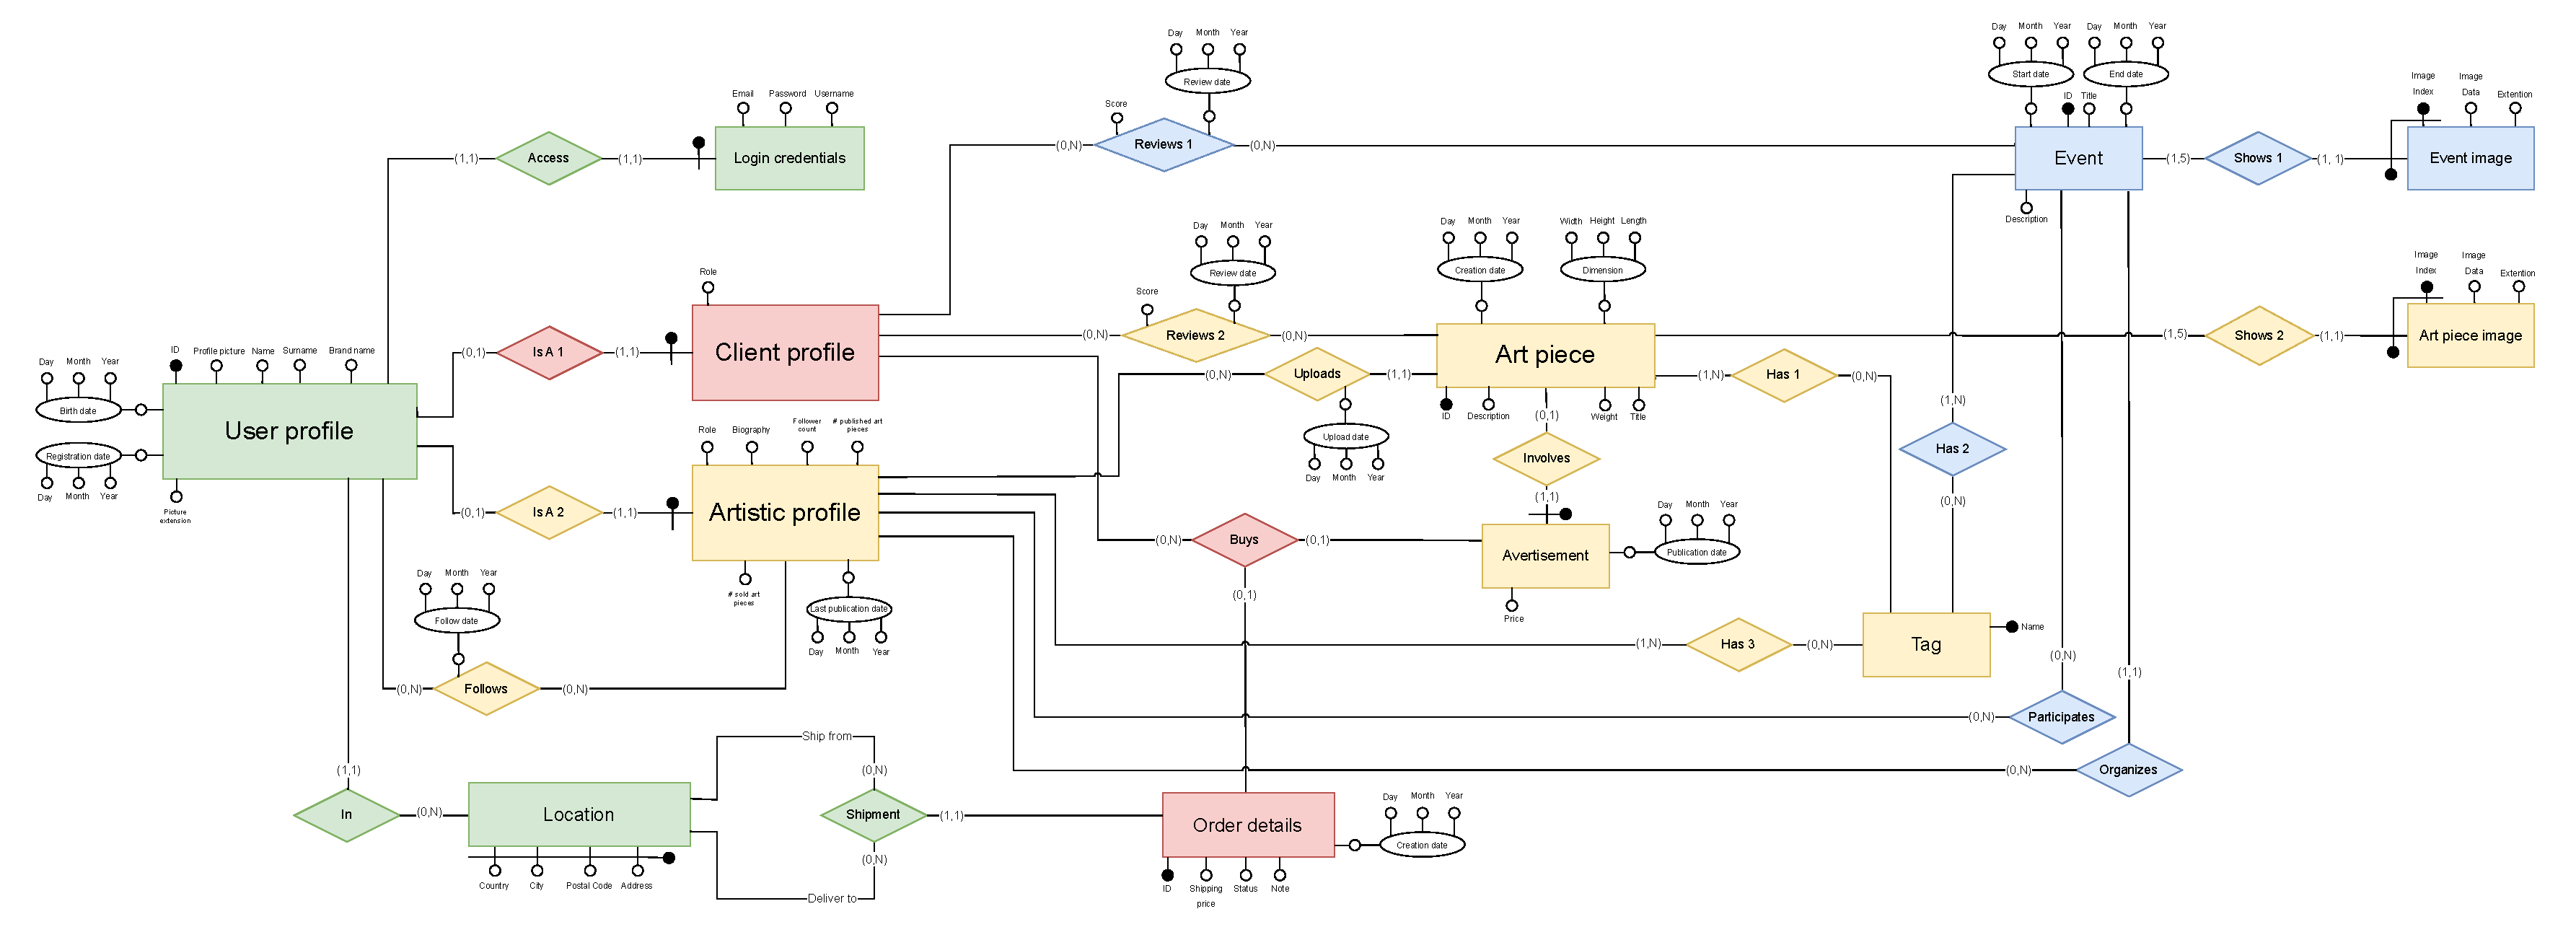
\includegraphics[width=1\linewidth]{images/ERschema.pdf}
\end{figure}

%Describe here your ER schema

The entity-relationship contains 12 main entities:
\begin{itemize}
    \item \textbf{User profile:} each user has, as primary key, an ID generated using UUID. For each user we also record
    a profile picture (of type byte array) with its extension (custom enumeration), a name and a surname which
    are of type char with variable length (up to 50 characters), a birth date (of type date) and a registration
    date (of type date). An optional brand name, only available to business users and art galleries, can be added
     as a char with variable length (up to 50 characters), for all other users it must be null.
    \item \textbf{Login credentials:} each user must have credentials to log in. This entity uses a foreign primary key 
    which is the primary key of the User profile and is used to save an email as char with with variable length 
    and a custom domain, a username as a char with variable length (up to 30 character) and a password as a char
     with variable length and a custom domain.
    \item \textbf{Location:} each location has a compound primary key which comprises the country which is a char with 
    variable length (up to 30 characters), the city which is a char with variable length (up to 30 characters), the
     address which is a char with variable length (up to 254 characters) and the postal code which is a char with 
     variable length (up to 10 characters).
    \item \textbf{Client profile:} is a subclass of the User profile entity which is used to represent generic users and 
    business users. This entity uses a foreign primary key which is the primary key of the User profile. It has a
     role (custom enumeration) which is used to discriminate between the two roles.
    \item \textbf{Artistic profile:} is a subclass of the User profile entity which is used to represent artists and art 
    galleries. This entity uses a foreign primary key which is the primary key of the User profile. It has a role 
    (custom enumeration) which is used to discriminate between the two roles, a 
    a biography (of type text), a follower count, number of sold art pieces, number of sold art pieces, which are
    all integers with auto-increment and decrement, a last published art piece (of type date) with auto update.
    \item \textbf{Art piece:} each art piece has, as primary key, and ID generated using UUID. For each art piece we 
    reference the ID of the author (which must be an artist) using a foreign key and we save the title of type char
    with variable length (up to 50 characters), a description (of type text), the weight (of type float), the width, 
    height and length (all of type float) and the publication date (of type date).
    \item \textbf{Art piece image:} an art piece image has a compound primary key made by the foreign primary key of the art 
    piece and a smallint index. The image has a field for the data (of type byte array) and one for the extension (
    custom enumeration).
    \item \textbf{Advertisement:} an art piece can have an associated advertisement, which has a foreign primary key which 
    is the primary key of the art piece. An advertisement contains the price (of type numeric) and the publication
    date (of type date).
    \item \textbf{Order details:} an order has, as primary key, an ID generated using UUID. For each order we reference the 
    shipping departure and arrival location using a foreign key and we save the shipping price (of type numeric), the 
    status (custom enumeration), a note as char with variable length (up to 254 characters) and the creation date (of 
    type date).
    \item \textbf{Event:} each event has, as primary key, an ID generated using UUID. For each event we reference the 
    the ID of the organizer (which must be an art gallery) using a foreign key and we save the start date (of type
    date), the end date (of type date), the title of type char with variable length (up to 50 characters) and a 
    description (of type text).
    \item \textbf{Event image:} an event image has a compound primary key made by the foreign primary key of the event and a 
    smallint index. The image has a field for the data (of type byte array) and one for the extension (custom 
    enumeration).
    \item \textbf{Tag:} each tag has, as primary key, a name which is a custom enum. It also has a cathegory (custom enumeration)
     to differentiate bewteen artist tags, art pieces tags and event tags.
\end{itemize}